% This is samplepaper.tex, a sample chapter demonstrating the
% LLNCS macro package for Springer Computer Science proceedings;
% Version 2.20 of 2017/10/04
%
\documentclass[runningheads]{llncs}
%
\usepackage{graphicx}
% Used for displaying a sample figure. If possible, figure files should
% be included in EPS format.
%
% If you use the hyperref package, please uncomment the following line
% to display URLs in blue roman font according to Springer's eBook style:
% \renewcommand\UrlFont{\color{blue}\rmfamily}

\begin{document}
%
\title{Data Driven Charging Station Placement}
%
%\titlerunning{Abbreviated paper title}
% If the paper title is too long for the running head, you can set
% an abbreviated paper title here
%
%
\maketitle              % typeset the header of the contribution
%
\begin{abstract}
With the development of electric vehicles, there comes a great need of charging stations for the recharging demand. However, where to locate a station and what are the main elements that operators should take into account when planning a setting, are still bothering problems that wait to be solved. In a common view, a better place to set a station ought to gurantee a relatively higher use rate of that station. Therefore, the problem changes into how to gain a higher use rate, and what are the factors that have important impact on it. In this paper, we propose a Feature To Explain LSTM(FTE-LSTM) framework of use rate prediction for charging stations and analyze the feature importance. The approach proposed in this paper takes both station's geographical information, such as longitude, latitude, surrounding Point of Interests(POIs), and working elements including price, AC/DC type and private or public to use, into consideration. After prerocessing, we seperate our datasets into urban area, suburb area and different time frames including total time, weekday, weekend, morning, evening. We evaluate our method in two tasks, including districts use\_rate prediction and time frames use\_rate prediction, aiming to classify what the level of a charging station's use rate is in different area districts and during different time periods. After classification work, we conduct the feature importance ranking for all the tasks to find out the inner relationships between features and accuracy, so that we can learn stations' placement hobbies. Experimental results show that our method performs well in classification accuracy and feature importance ranking, which demonstrates that selected featrues especially important POIs play important roles in use rate of charging stations.

\keywords{charging station \and use rate \and POIs \and feature importance}
\end{abstract}
%
%
%
\section{Introduction}
An electric vehicle charging station, also called EV charging station is an element in an infrastructure that supplies electric energy for the recharging of electric vehicles, such as plug-in electric vehicles and plug-in hybrids. At home or work, some electric vehicles have onboard converters that can plug into a standard electrical outlet or a high-capacity appliance outlet. 

However, in most cases, others require a charging station that provides electrical conversion, monitoring, or safety functionality. These stations are also needed when travelling, and many support faster charging at higher voltages and currents that are available from residential EVSEs. Public charging stations are typically on-street facilities provided by electric utility companies or located at retail shopping centers and operated by many private companies.


EVs in China is experiencing an overall growth in the past few years, which directly results in the massive construction and modification of charging stations and current road networks.  However, the cost of construction of charging stations is considerable and are often very costly or even impracticable to reallocate. This raise the question of how to select the locations for building the charging stations. In a typical view, a charging station no matter where it is located, its 'success' is often determined by the use rate of a station. Fig.\ref{fig1} shows an operator's stations use rate distribution in Shanghai, from which we can observe some hotspots where stations are frequently used.

\begin{figure}[!htp]
	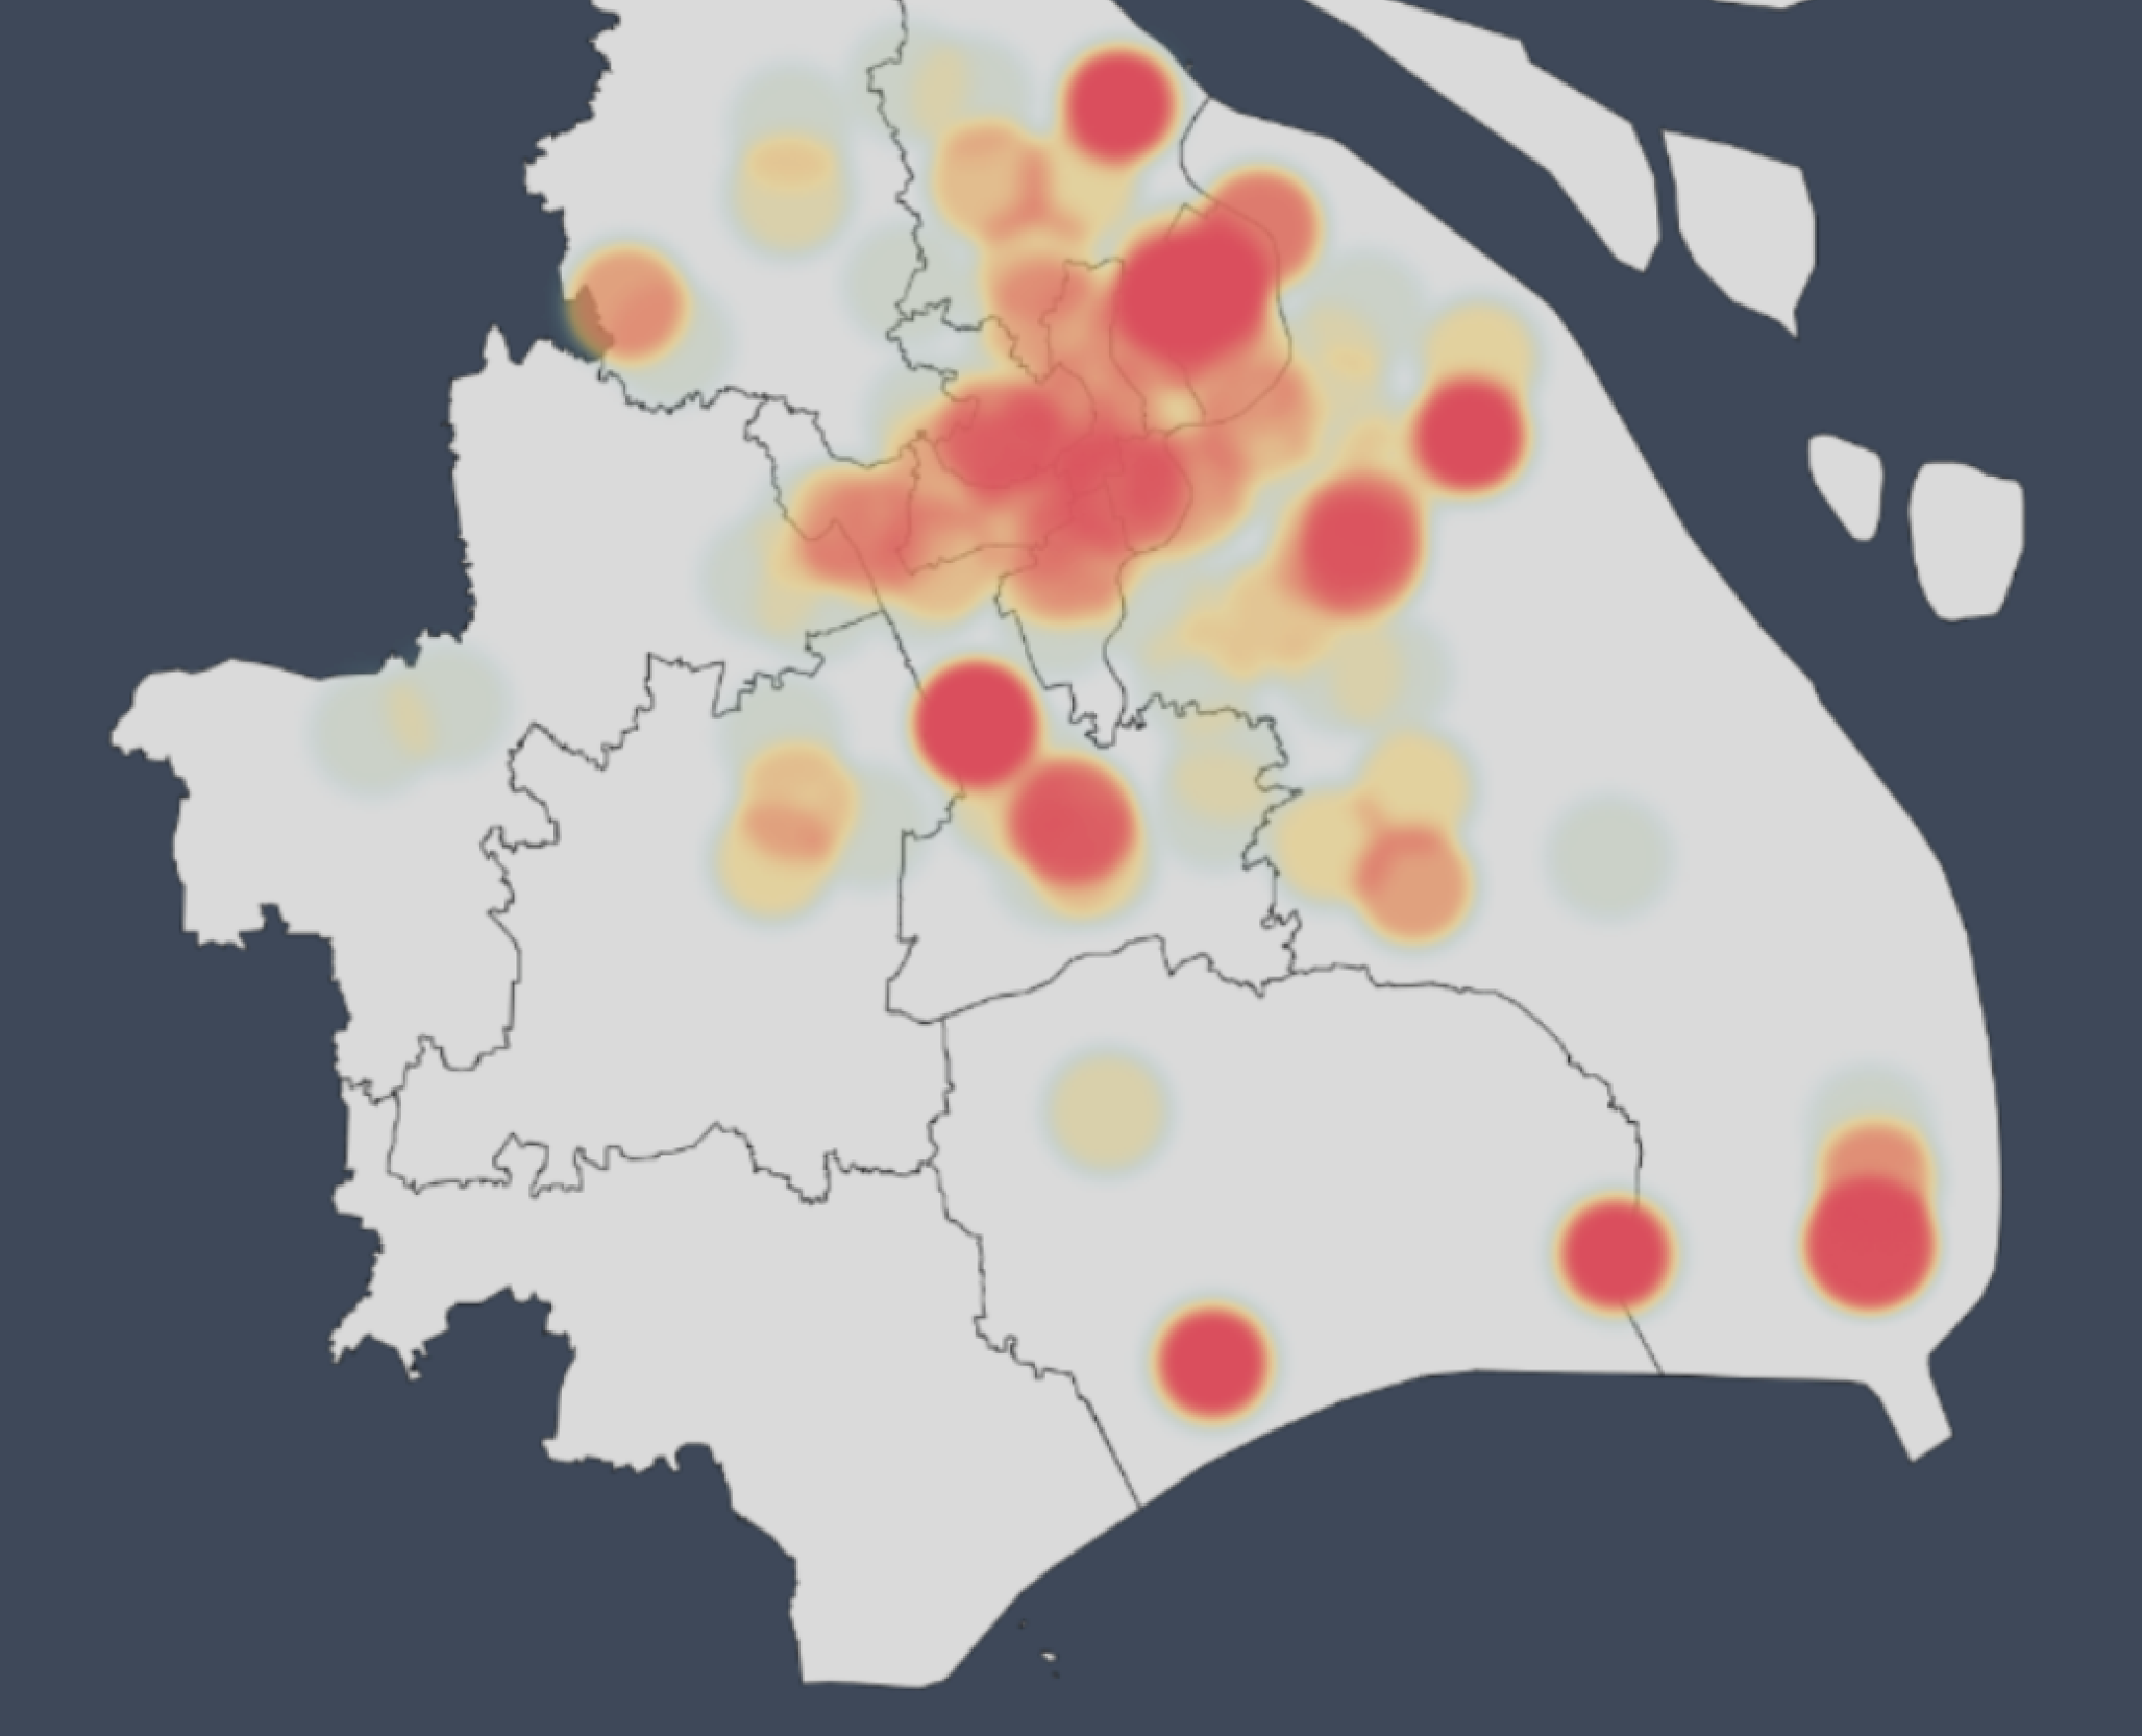
\includegraphics[width=\columnwidth]{./figures/rate.pdf}
	\centering
	\caption{Use Rate Distribution of An Operator's Stations in Shanghai, China. The deeper the color is, the more frequently charging stations are used in this area.}
	\label{fig1}
\end{figure}  

Traditional location selecting methods are mainly about sharing bikes. They focus much more on bikes or stations' spatio-temporal features. \cite{Bao:2017} makes use of sharing bikes' trajectory data for bike lane planning. \cite{Li:2018:DBR} clusters stations into groups according to their status and implements a reinforcement learning.

In order to help with charging station setting strategies, we explore a Feature To Explain LSTM (FTE-LSTM) framework to classify stations into three use rate levels in urban-suburb districts and various time frames, furthermore, to classify specific use rate values into urban or suburb aera, using features like georaphical information as well as other working elements. After classification work, we rank the feature importance correlated to each result. We set 4 time frames in total, they are weekdays, weekends, mornings, evenings. As for features, we choose longitude, latitude, Point of Interests(POIs), charging price, AC/DC charging types and whether a station is private or public to use.

We make use of an operator's charging station data in Shanghai and  have kept collecting the use rate values for about a month, then we seperate the whole use rate dataset into urban or suburb districts and various time frames that we have already planned. At the same time, we also collect important featrure data as formerly said. Both of the two datasets require a data cleaning procedure, in order to filter some invalid data and outliers, and to fill in missing values. Furthermore, we make detailed analyses on features that we confirm to have significant impact on station's use rate.

We evaluate our method on districts use\_rate prediction and time frames use\_rate prediction. In each district and time frame, with features put into it, the models will tell what level of use rate that a station is. Furthermore, we rank the feature importance to evaluate each features's impact on the prediction accuracy. Experimental results show that our chosen features especially importance POIs do have great influence on stations use rate, which can bring operators some enlightments on location selection for station construction.

In summary, the contributions of this work are listed as follows:
\begin{itemize}
	\item We propose a Feature To Explain LSTM (FTE-LSTM) framework to predict what level of use rate a station is and which district a station belongs to, based on operator's charging station data and important features.
	\item We make detailed analyses on both stations data and features data to obtain basic information and find the relationships between station's use rate and those features.
	\item We evaluate our method on two classification tasks, and it performs well in both classification accuracy and feature importace ranking.
\end{itemize}
The rest of this paper is organized as follows: Section 2 gives definition of the problem and illustrates an overview of our work. Section 3 reviews some related work done before. Section 4 describes feature analyses and work on data processing. Section 5 provides experiments on three tasks and the results of classification and ranking work. In Section 6, we draw a conclusion to the paper and make discussions on future work.

\section{Design Overview}
There are many elements that affect location selection for charging stations when operators make the decision. In this paper, we hold that use rate of a station is the key factor which determines the 'success' of the station. Therefore, the original problem turns into how to get a higher use rate and what are the factors behind it. 

The main objectives of our work is three-fold. First, we aim to explore some important featrues that have great impact on use rate of a station using spatio-temporal data of operator's charging station data. Second, we propose to study stations' different 'behaviours' in different districts like urban area or suburb area as well as in diverse time frames. Finally, we aim to predict that one station is of what level of use rate, according to its georaphical information and working elements. Furthermore, for each calssification task, we conduct a feature importance ranking to find out how these features impact on stations use rate.

Based on all the analyses mentioned above, we propose the Feature To Explain LSTM (FTE-LSTM) framework to help with use rate prediction for charging stations and provide feature ranking . Fig.\ref{fig2} gives the overall data processing and learning pipelines of our work.

\begin{figure*}[!htp]
	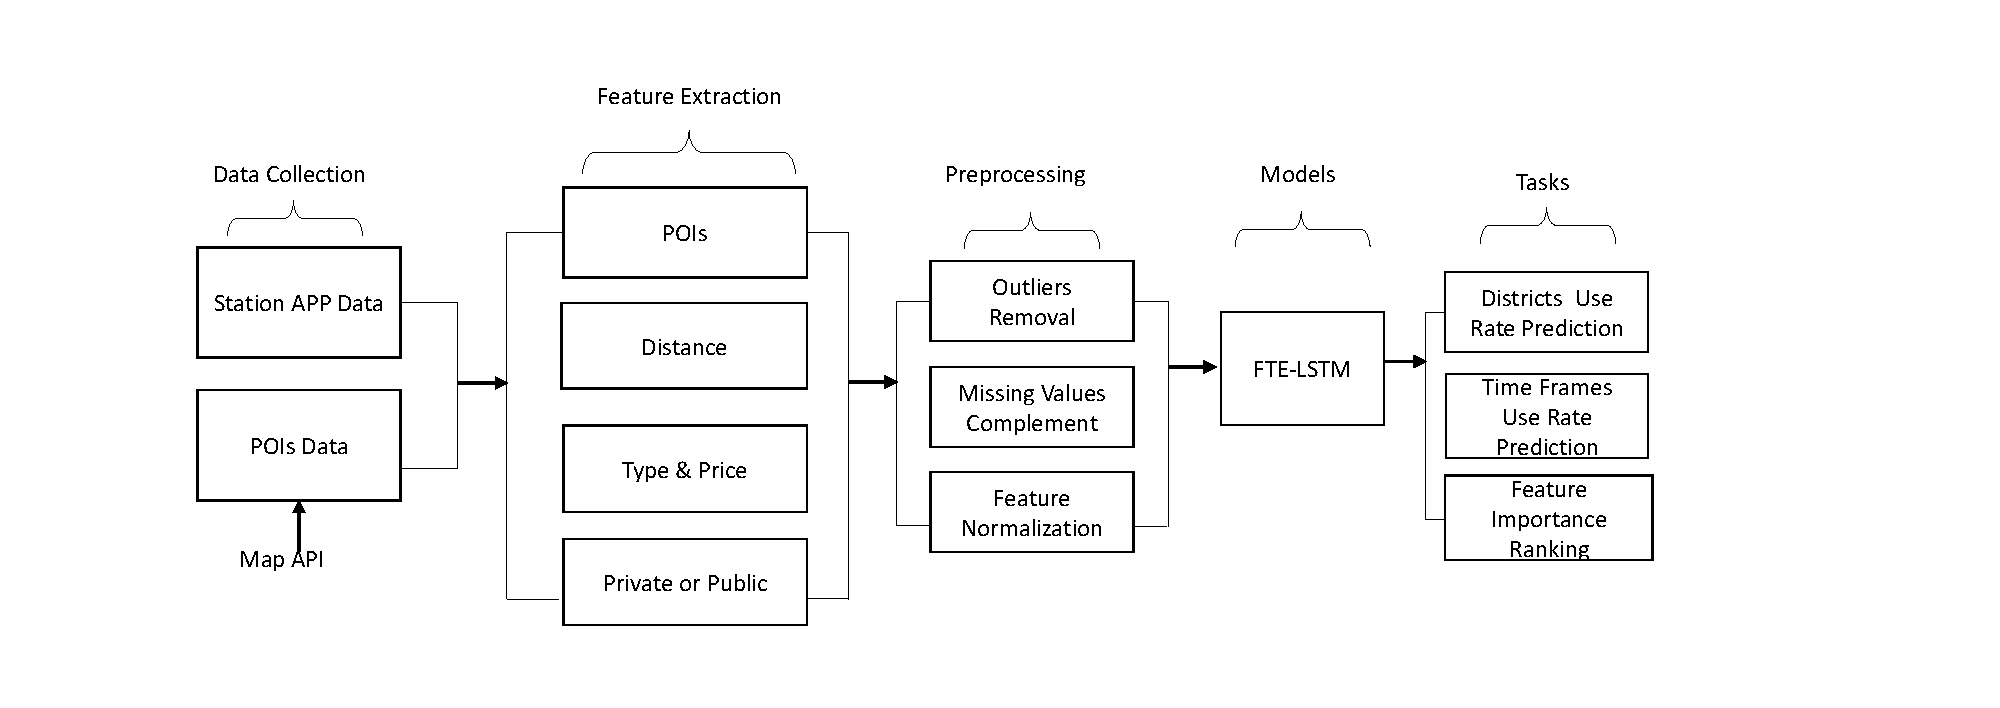
\includegraphics[width=\columnwidth]{./figures/pipeline.pdf}
	\centering
	\caption{Overall Pipelines of Data Processing and Learning}
	\label{fig2}
\end{figure*}

\section{Related Work}

Hence, we studied the optimization problem of how to deploy charging stations. Existing works \cite{Bao:2017,Liu:2018:DSB,Yang:2016:MMP,Li:2018:DBR,Liu:2016:RB} mainly fall into the domain of bike-sharing. The objective is to find a proper strategy for bike lane planning or sharing-bikes reposition, in order to help with a more resonable city planning. \cite{Bao:2016,Chen:2011,Jiang:2016,Li:2016}, they are usually based on sharing-bikes' trajectory data, which is full of spatio temporal information. \cite{Bao:2017} provides a data-driven apporoach to deal with bike lane construction problem. It takes government constraints of planning bike lanes, such as budget limitations, construction convenience and bike lane utilization into consideration to formulate the problem. Furthermore, the problem is proved to be NP-hard so that they propose a greedy network expansion algorithm to help work out a scalable and approximate solution to bike lane planning problem. The approach performs well in the given problem, however it doesn't make use of learning models. \cite{Li:2018:DBR} introduces a reinforcement learning algorithm to help solve the problem of repositioning sharing-bikes. First it uses an inner-balance clustering algorithem to cluster stations into groups, then the reinforcement learning algorithm is conducted in each group to learn a reposition policy. They make a good use of spatio-temporal data while don't take advantages of useful surrounding and station-self features. \cite{Liu:2016:RB} proposes a new method using weighted K-Nearest-Neighbor to predict bike-sharing stations' pick up demand and a new model to predict drop off demand, it also study on stations clustering to simplify the problem. With these steps they explore a useful way to optimize bike-sharing system's rebalancing operations.

Current works of location selection are usually based on the flow prediction of a single station. Futhermore, they mainly rely on the historical data. \cite{Yang:2016:MMP} introduces a model for bicycle mobility prediction. It relis on historical bike-sharing data and a per-station basis with sub-hour granularity. It makes use of the randonm forest prediction model to implement their experiments and obtain a rather good result. \cite{Liu:2016:CTP} gives an optimization to this problem. Its way for traffic prediction no longer focuses on the history data only, but can use location-based socail media to collect a much larger area of the traffic data for predicting traffic conditions. Other work on urban life prediction take advantages of spatio temporal data and useful machine learning algorithms \cite{Hoang:2016,Li:2018,Liao:2018:DSL:3219819.3219895,Liu:2016:CTP,Shen:2018:SNS,Zhou:2018:DLP:3219819.3219929}. \cite{Zhou:2018:DLP:3219819.3219929} make use of users' geographical check-in information in Wechat and dig into the rich spatio temporal representations behind users' activity at cultural venues. Then the authors propose a latent Dirichlet allocation model to identify latent patterns of urban cultural interactions, in order to help with urban cultural planning and investment optimazation. \cite{Shen:2018:SNS} is also a good example of prediction model for spatio-temporal mobility event. It encodes each POI's spatio and temporal dependencies rather than neglect the correlations between POIs.

\cite{lime} introduces a framework to explain the prediction procedures of any classifier. It calculates each feature's 'contribution score' in classification accuracy to tell us how the classifier works on features and get the final results. This work enlightens us a lot, and we follow the main idea to design our framework.

In this paper, we also focus on stations' spatio temporal data and make use of machine learning algorithms to help with our analyses. Then we conduct feature importance ranking according to each feature's 'contribution score' in final results.

\section{Methodology}
\subsection{Feature Extraction}


\subsubsection{Point Of Interest}
To the prosperity of Shanghai, there are so many points of interest(e.g., shopping malls, schools. estates, companies, etc.) located in the city.  Understanding the purpose of the trip by each person who participates in charging system will help us to analyze the use rate prediction. So, we need to extract the POI around each existing charging station. There are a lot of POIs in Shanghai. The POIs are very close to each other. We set a radius around each station and then collect the POIs within the radius. Based on our experiment, choosing a radius as 300 meters is proper. In our work, we get 80 different types of POI totally. Some of the POIs are very similar to each other. Therefore, we group 80 POIs in further step. By grouping POIs, we get 10 groups at last. Table.\ref{tab1} gives the groups and POIs in detail.

\begin{table}[!htbp]
	\caption{Groups of POIs}
	\begin{center}
		\begin{tabular}{|l|p{9cm}|}
			\hline
			Group & Points of interests\\
			\hline
			Food & chinese \& foreign restaurant, snack bar, cake \& dessert shop, cafe, bar\\
			\hline
			Hotels & star hotel, express hotel, apartment hotel\\
			\hline
			Shopping & shopping centers, department stores, supermarkets, convenience stores, home building materials, home appliances digital, shops, markets\\
			\hline
			Education & institutions of higher learning, middle schools, primary schools, kindergartens, adult education, parent-child education, special education schools, study agencies, research institutions, training institutions, libraries, science and technology museums\\
			\hline
			Cultural venue & press and publication, radio and television, art groups, art galleries, exhibition halls, cultural palaces\\
			\hline
			Medical & general hospitals, specialist hospitals, clinics, pharmacies, medical examination institutions, nursing homes, emergency centers, disease control centers\\
			\hline
			Car service & car sales, car repair, car beauty, auto parts, car rental, car inspection field\\
			\hline
			Transportation & airport, railway station, subway station, subway line, long-distance bus station, bus station, bus line, port, parking lot, refueling station, service area, toll station, bridge, charging station, roadside parking space\\
			\hline
			Estates & Office building, residential area, dormitory\\
			\hline
		\end{tabular}
		\label{tab1}
	\end{center}
\end{table}

\subsubsection{Distance}

In use rate prediction, we need to consider distance. People will not choose to park their electric cars for charging if the destination they planned to go is far away. In the system, a station with nearer distance to metro stations, financial centers and major functional buildings would easily be used more often. We select the nearest distance to the following to be the distance we considered as features: company, estate, hospital, metro station, shopping center and university. Fig.\ref{fig4} shows the total count of these important 'distance' POIs, from the figures we can see that these features almost satisfy the long tail distribution, which will be normalized in later work, see Preprocessing part.

\begin{figure}[!htbp]
	\begin{tabular}{cc}
		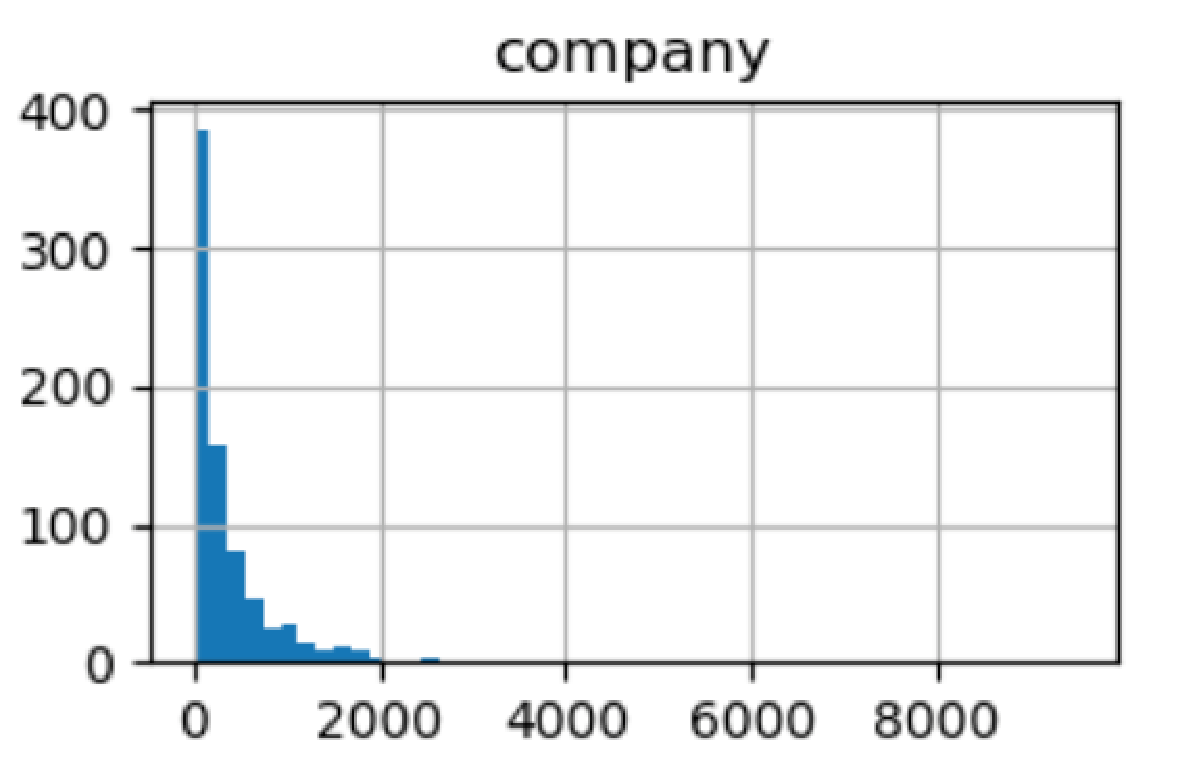
\includegraphics[width=0.45\columnwidth]{./figures/company.pdf} &  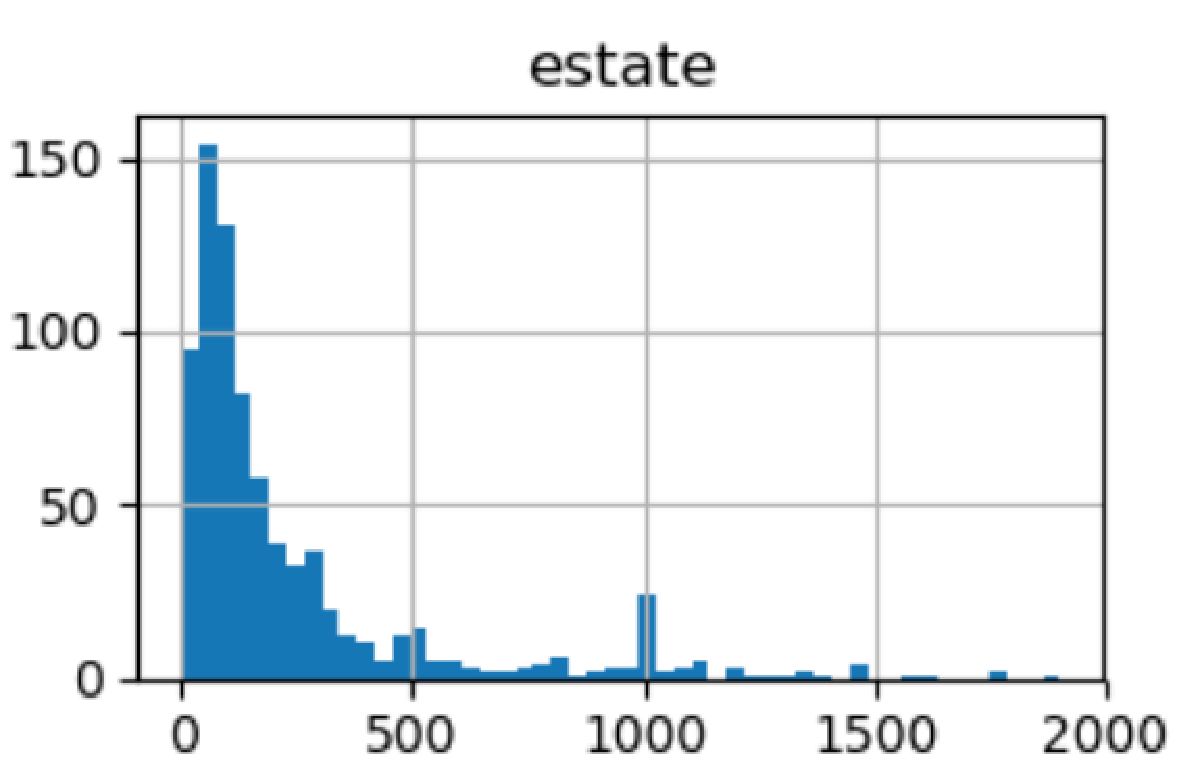
\includegraphics[width=0.45\columnwidth]{./figures/estate.pdf} \\
		(a) Company & (b) Estate \\[6pt] 
		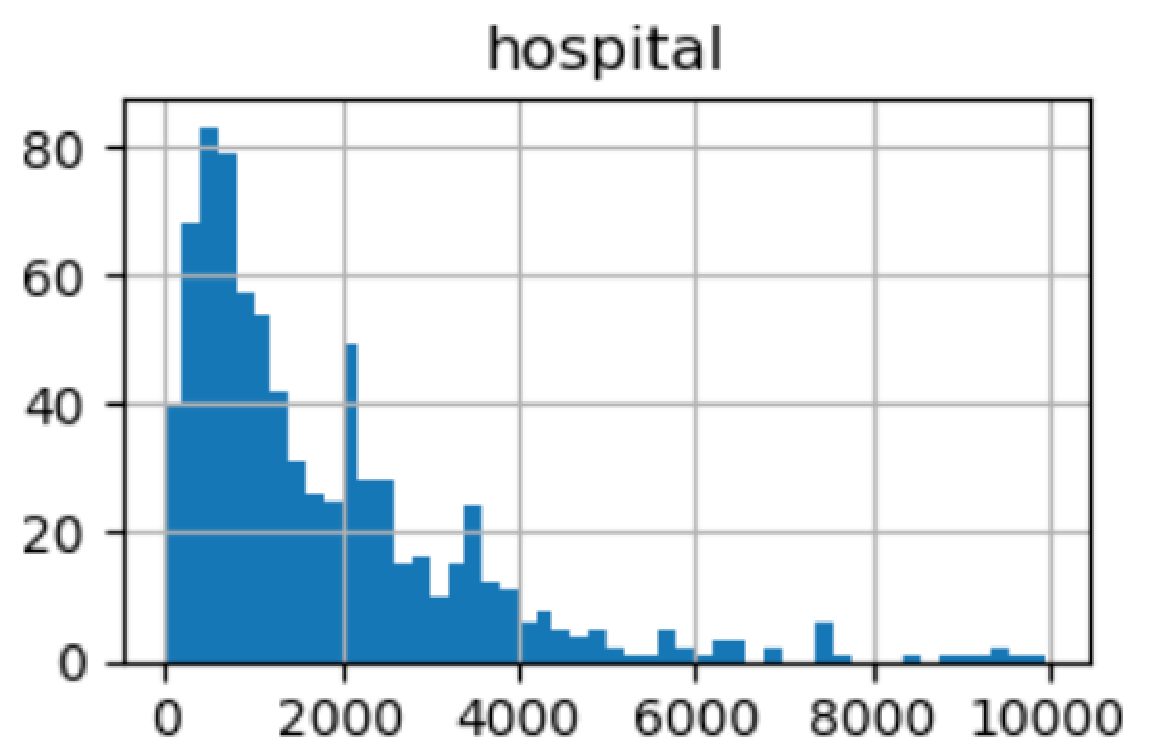
\includegraphics[width=0.45\columnwidth]{./figures/hospital.pdf} &
		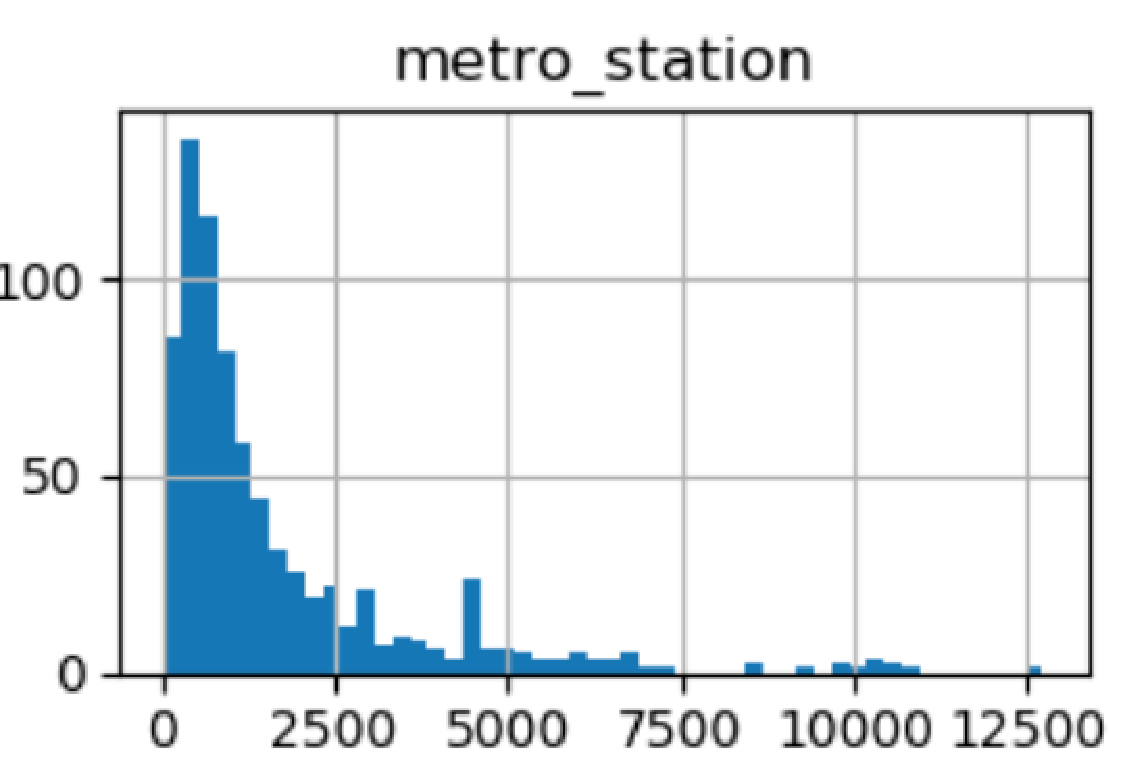
\includegraphics[width=0.45\columnwidth]{./figures/metro.pdf} \\
		(c) Hospital & (d) Metro Station \\
		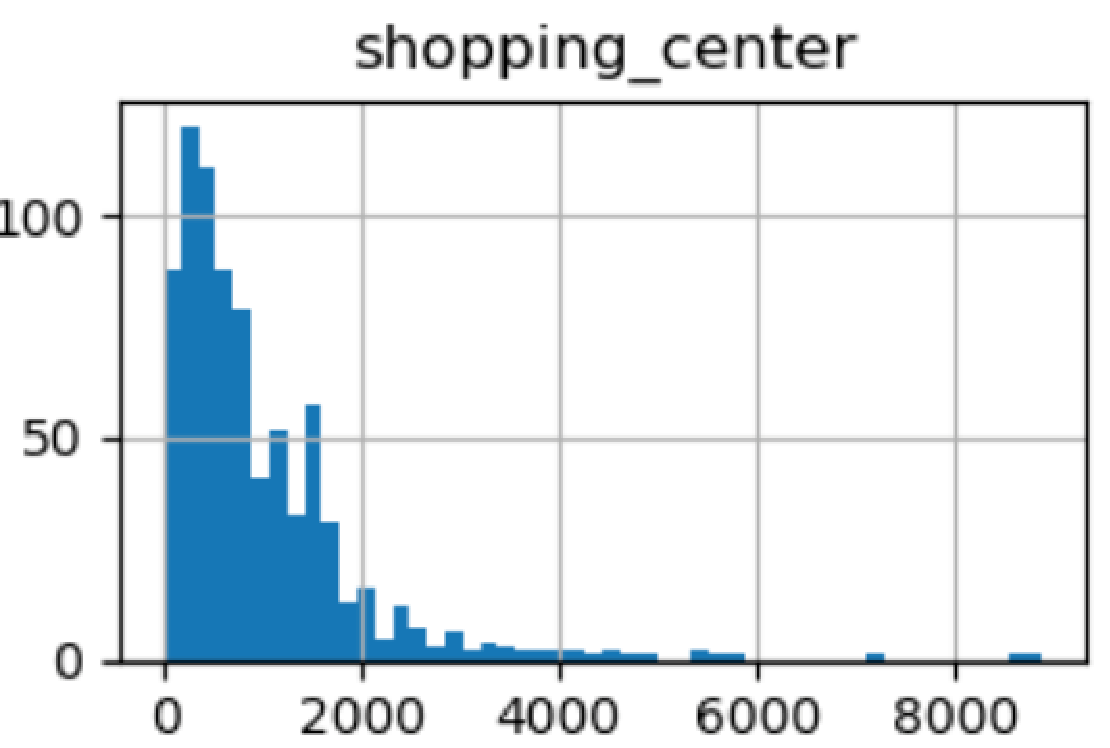
\includegraphics[width=0.45\columnwidth]{./figures/shop.pdf} 
		&
		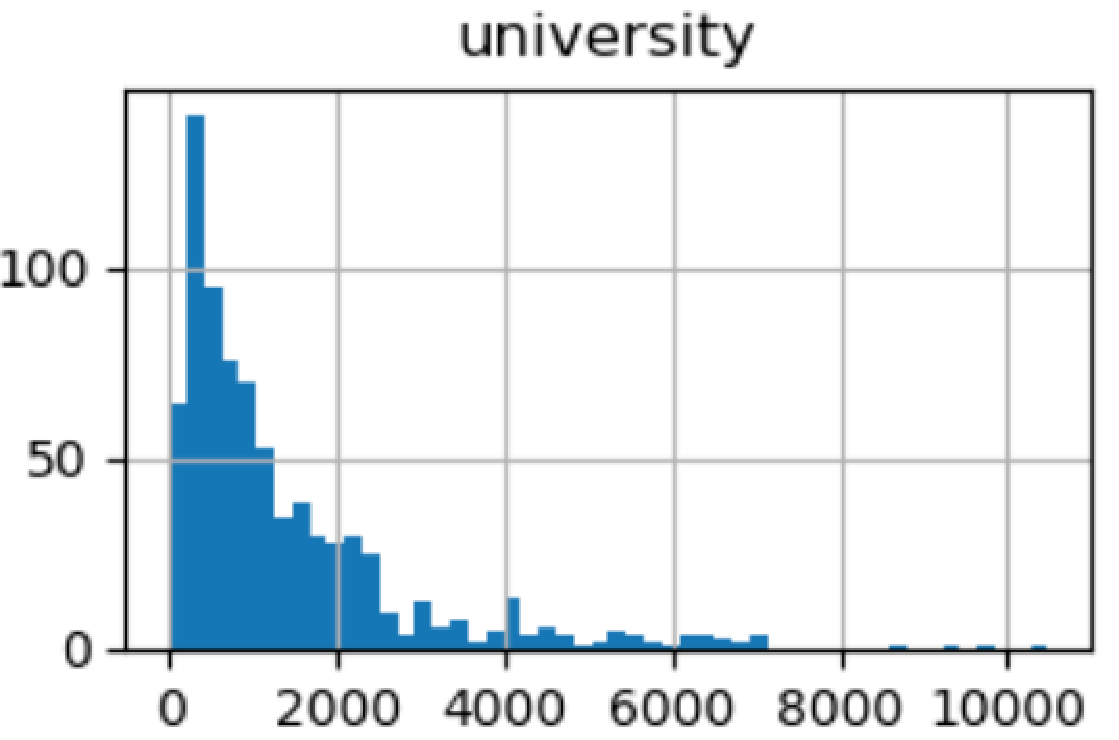
\includegraphics[width=0.45\columnwidth]{./figures/university.pdf} \\
		(e) Shopping Center & (f) University
	\end{tabular}
	\centering
	\caption{Count of Important POIs}
	\label{fig4}
\end{figure}

\subsubsection{Type \& Price}
By futher digging into the data, we find that there is a 0.3 correlation between price for charging and the use rate. Since there are two types of charging ports: DC and AC. We would include the number of ports and the price of both types in a charging station as one of its feature. Fig.\ref{fig5} shows the number of AC/DC type of stations's charging ports, as well as each type's charging cost fee. From the figures we observe that there are much more AC type charging ports than DC type ones, while the charging cost fee of them two are almost the same.

\begin{figure}[!htbp]
	\begin{tabular}{cc}
		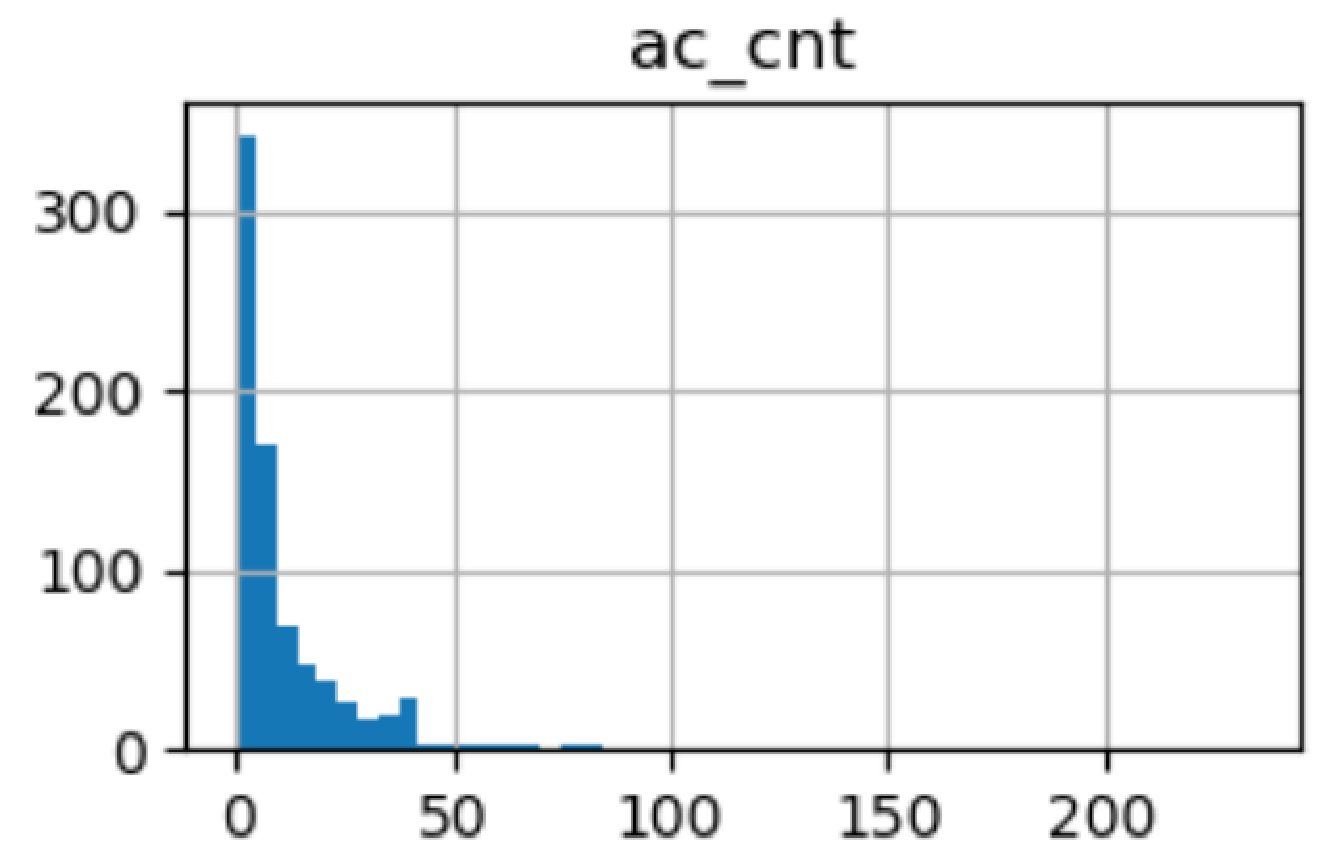
\includegraphics[width=0.45\columnwidth]{./figures/ac_cnt.pdf} &  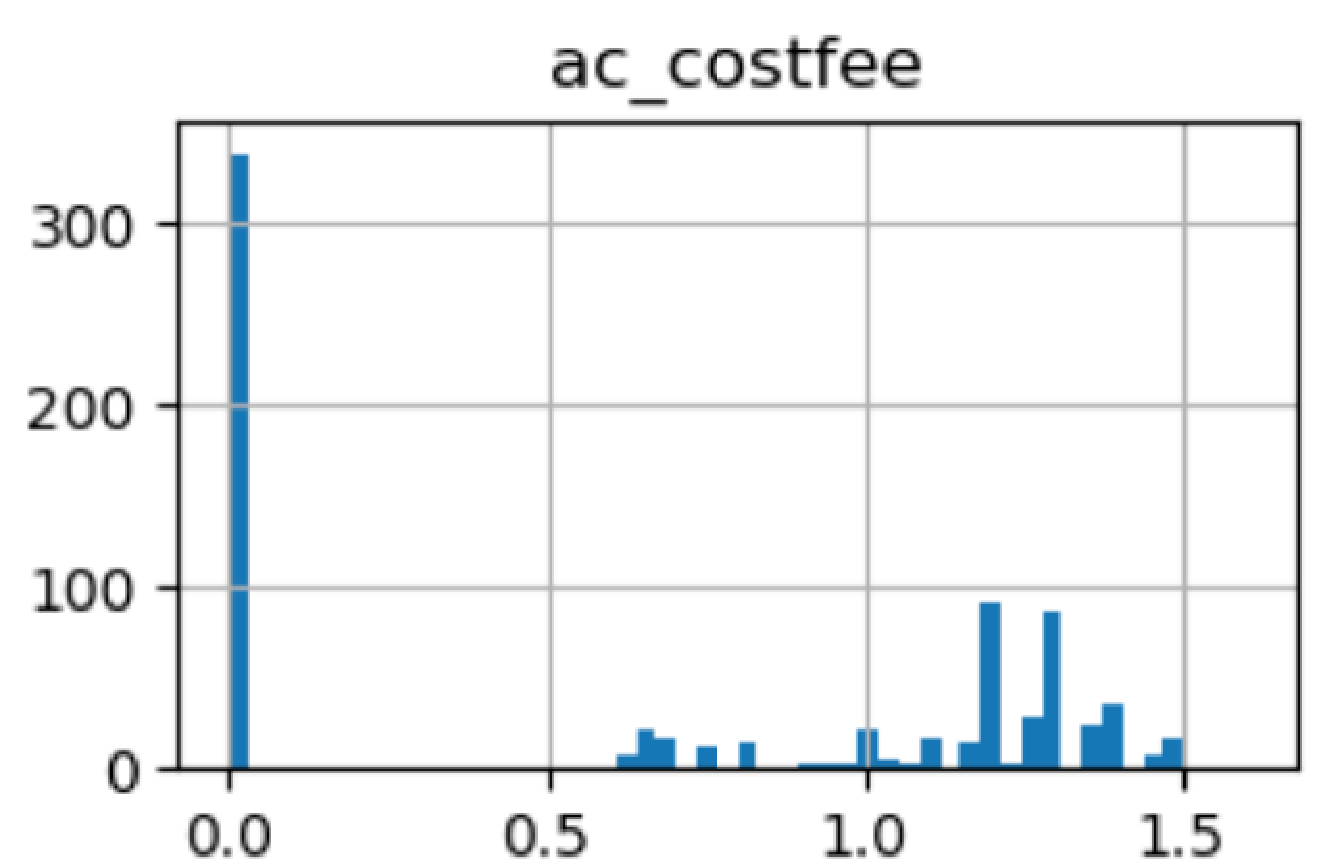
\includegraphics[width=0.45\columnwidth]{./figures/ac_fee.pdf} \\
		(a) AC\_Count & (b) AC\_Fee \\[6pt] 
		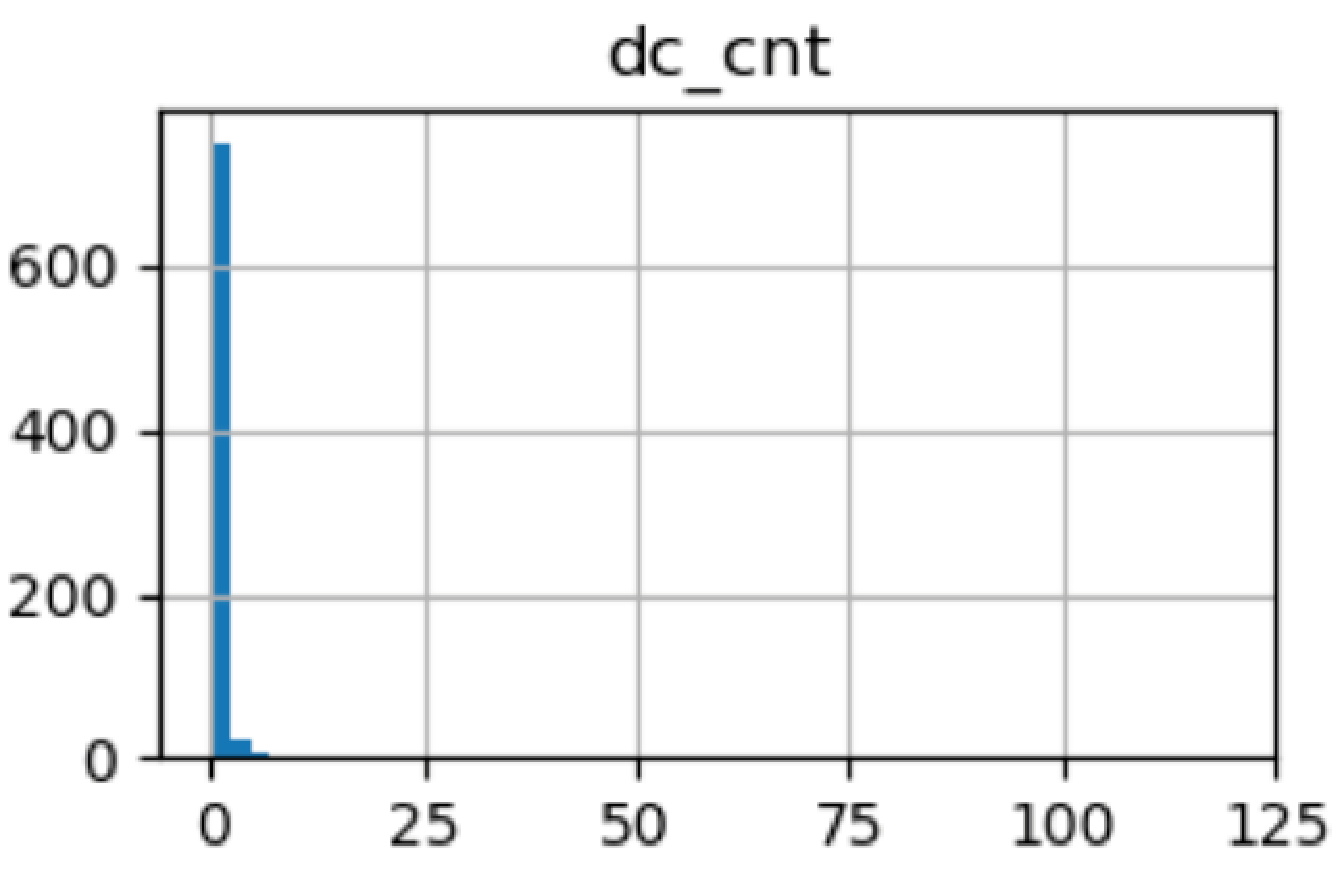
\includegraphics[width=0.45\columnwidth]{./figures/dc_cnt.pdf} &
		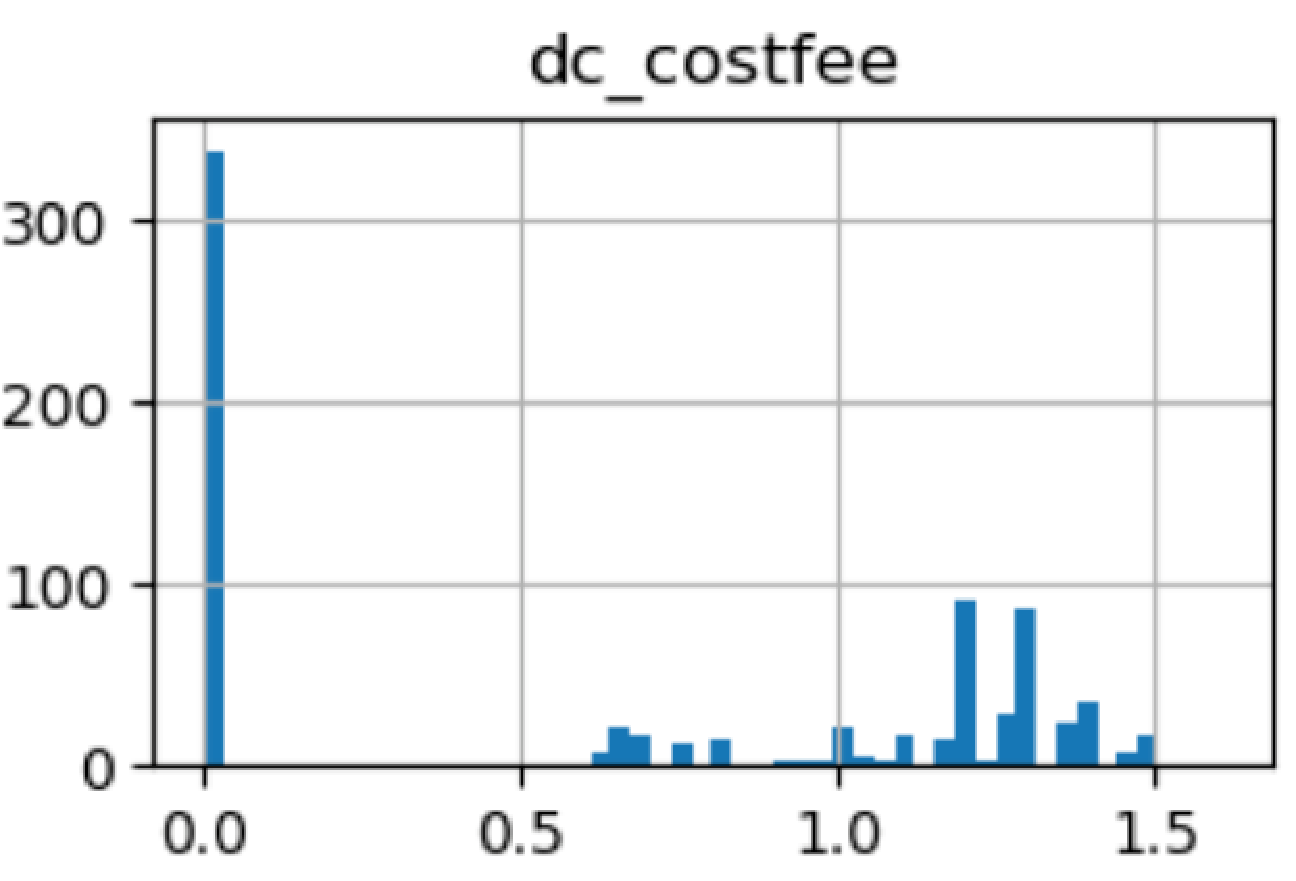
\includegraphics[width=0.45\columnwidth]{./figures/dc_fee.pdf} \\
		(c) DC\_Count & (d) DC\_Fee
	\end{tabular}
	\centering
	\caption{Charging Stations Types and Charging Cost Fee}
	\label{fig5}
\end{figure}

\subsubsection{Private or public}
By observing the data we've collected, it can be seen that most of the charging stations are private charging stations, which means they are typically used by electric buses and rent cars, or used by specific companies for their employees, accounting for over 70\% of the total charging stations. Also, since the private are used by more regular users(e.g., buses, companies employees), its use rate are 5\% higher compared to public ones. This alongside other observations will be taken into consideration.

\subsection{Spatio Temporal Data}

\subsubsection{Ditricts}
There are 16 districts of station data in total,and for experiment, we separate them into two parts as urban area and suburb area. The final dataset for district prediction task contains the two parts of data, in urban part, 7 districts are included while in suburb part, 9 left districts are included.
\subsubsection{Time Frames}
In order to further study stations' use rate in different time periods, we set different time frames, including total time, weekday, weekend, daytime, evening time, morning\_rush hours, evening\_rush hours and travel\_hours, to help observe the use rate discrepancy during these phases. 

\subsection{Preprocessing}
\subsubsection{Data Cleaning}
The original dataset may exist some outliers and missing values, there should be a data cleaning procedure to deal with these invalid data. For outliers, if detected, we remove them from the dataset; for missing values, we use the median filling method to fill blanks with median values computed via 'Imputer' function.

\subsubsection{Feature Zooming}
In 'nearest important POIs', the value of each feature is over hundred, while in other features like 'dc cost fee', the mean value is just about 0.85 per hour. In order to achieve a better performance using machine learning algorithms, we take a feature zooming procedure to normalize feature values so that they can range in [0,1]. Different models may use different zooming strategies, which will be discussed in detail in experiment section. Fig.\ref{fig8} shows an example of the feature 'university' after normalization step.
\begin{figure}[!htp]
	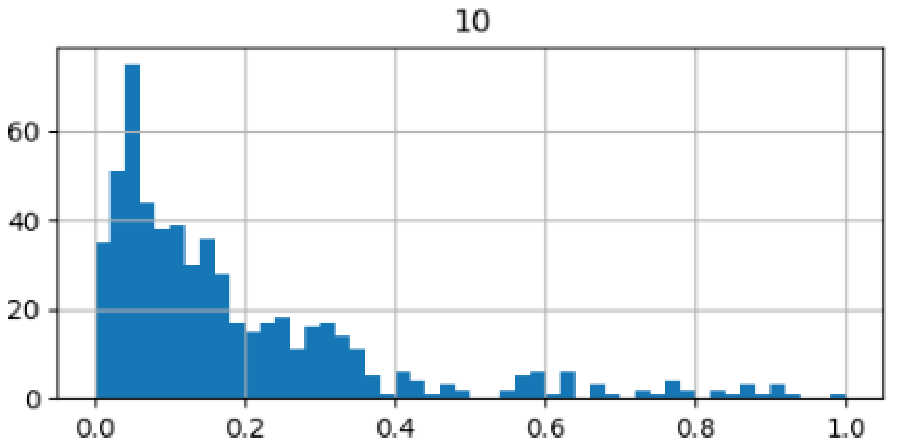
\includegraphics[width=\columnwidth]{./figures/uni.pdf}
	\centering
	\caption{An Example of Feature Normalization}
	\label{fig8}
\end{figure}
\subsection{Feature To Explain LSTM Framework}
For districts use\_rate prediction and time frames use\_rate  prediction tasks, we follow the general LSTM model\cite{LSTM} as the classifier to get the accuracy. To further understand the impact of given features on prediction accuracy, we conduct the feature importance ranking, using the ranking algorithm called Gradient Boosted Decision Tree(GBDT). For each feature, it first calculates feature importance for a single decision tree and then the feature importances are averaged across all the decision tress within the model to get the final 'contribution score' to do the ranking. We combine the LSTM classifier and ranking algorithm together to propose our Feature To Explain LSTM(FTE-LSTM) Framework for both classification tasks and explaining the feature importance.

\section{Experiments}
We compare the proposed FTE-LSTM with traditional classifiers including Random Forest and MLP in classification accuracy, and then provides the feature importance ranking of our model's result to find out the relationships between selected features and use rate.
\subsection{District Use\_Rate Prediction}
The task of district prediction aims to classify stations into high, middle or low use rate in urban and suburb areas of Shanghai. Because the use rate of charging stations range in [0,1), so we set three levels as labels for classification task. In detail, we set use rate from 0 to 20\% as low\_use\_rate; 20\% to 50\% as mid\_use\_rate; and over 50\% as high\_use\_rate.

We first separate our dataset into two parts: urban areas data and suburb areas data. After this operation, about 30\% of station data is in the urban one, and other 70\% of data is in the suburb one. Then, for each part, we randomly choose 80\% of the data as training set, and 20\% left as test set. We use mean average precision(MAP) as evaluation method which is commonly used in multilabel classification task.

Table.\ref{tab2} and Table.\ref{tab3} show the prediction accuracy of different models on urban areas data and suburb areas data. From the results we observe that our model outperforms the traditional classifiers in both urban and suburb parts.
\begin{table}[htbp]
	\caption{Evaluation results on urban prediction}
	\begin{center}
		\begin{tabular}{|l|l|}
			\hline
			Model & Accuracy\\
			\hline
			MLP & 74.35\%\\
			\hline
			Random Forest & 79.52\%\\
			\hline
			FTE-LSTM & \textbf{84.62\%}\\
			\hline
		\end{tabular}
		\label{tab2}
	\end{center}
\end{table}

\begin{table}[htbp]
	\caption{Evaluation results on suburb prediction}
	\begin{center}
		\begin{tabular}{|l|l|}
			\hline
			Model & Accuracy\\
			\hline
			MLP & 80.72\%\\
			\hline
			Random Forest & 78.31\%\\
			\hline
			FTE-LSTM & \textbf{85.74\%}\\
			\hline
		\end{tabular}
		\label{tab3}
	\end{center}
\end{table}
Then we conduct feature ranking in our model. Fig\ref{fig9} and Fig.\ref{fig10} are the ranking results in urban prediction and suburb prediction respectively. F0-F10 are the features correlated to type, dc\_costfee, ac\_costfee, parking\_fee, serve\_fee, company, estate, hospital, metro\_station, shopping\_center and university. And the higher score represents the higher importance. For both prediction tasks, we can see that the POI 'metro\_stations' plays the most significant role in stations' use rate, in urban area, use rate is influenced more by 'hospitals' than 'shopping\_centers' while in suburb, these two features are at the opposite position.
\begin{figure}[htbp]
	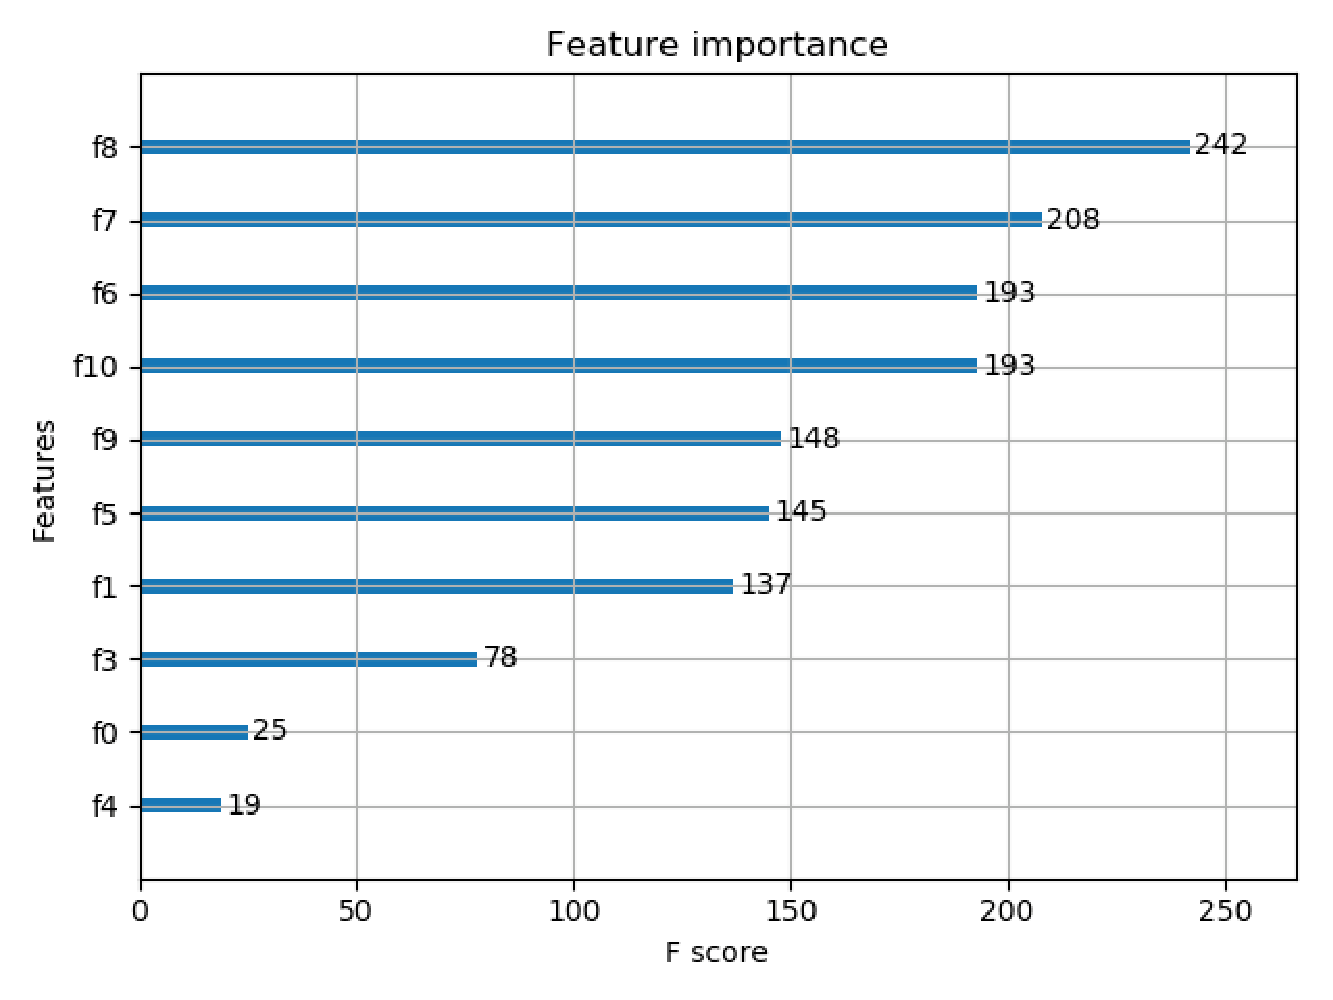
\includegraphics[width=0.7\columnwidth]{./figures/urban_rank.pdf}
	\centering
	\caption{Feature Importance of Urban Prediction}
	\label{fig9}
\end{figure}

\begin{figure}[!htp]
	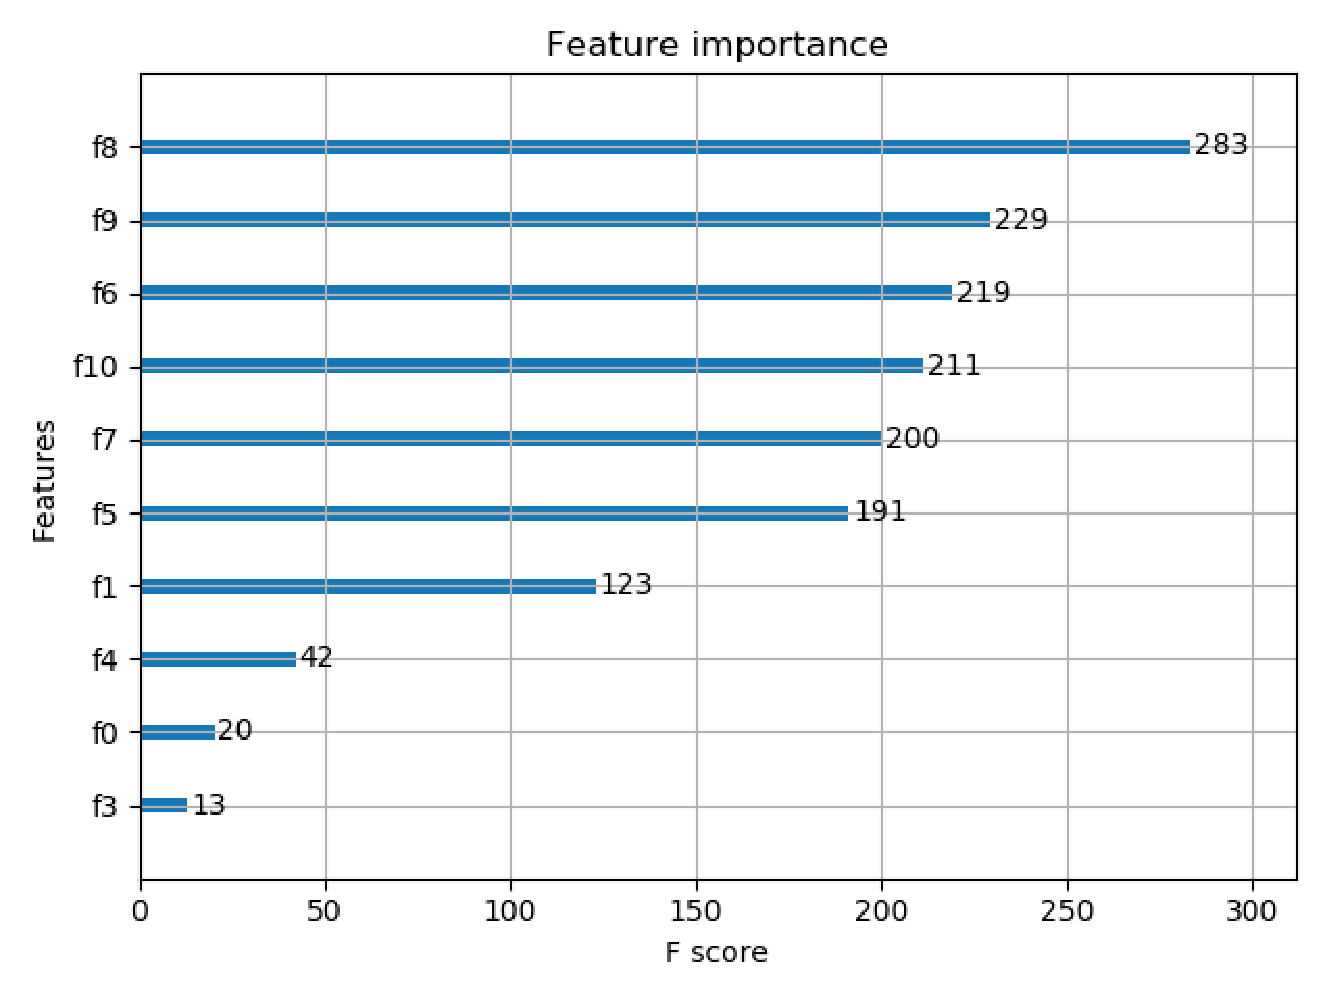
\includegraphics[width=0.7\columnwidth]{./figures/subur_rank.pdf}
	\centering
	\caption{Feature Importance of Suburb Prediction}
	\label{fig10}
\end{figure}
\subsection{Time Frames Use\_Rate Prediction}
Stations' use rate in different time frames is a more concerned problem we want to explore. According to time frames partition mentioned in Section 4, we also separate station data into 4 time frames: weekday, weekend, morining, evening. In this task, features like POIs, charging port type and charging price still stay the same, while the use rate itself will vary in different time frames, so that the level of use rate, also the classification labels will differ from each time frame dataset. After preprocessing, we also randomly choose 80\% of valid data as training set, and the left as test set.

Table.\ref{tab4} shows the accuracy of different models on time frames data. 
\begin{table}[htbp]
	\caption{Evaluation Results On Time Frames Prediction}
	\begin{center}
		\begin{tabular}{|l|l|l|l|l|}
			\hline
			Model & Weekday & Weekend & Morning & Evening\\
			\hline
			MLP & 76.72\% & 92.13\% & 77.59\% & 81.90\%\\
			\hline
			Random Forest & 72.41\% & 90.27\% & 74.14\% & 83.62\%\\
			\hline
			FTE-LSTM & \textbf{82.23\%} & \textbf{96.55\%} & \textbf{85.41\%} & \textbf{88.76\%}\\
			\hline
		\end{tabular}
		\label{tab4}
	\end{center}
\end{table}

In order to evaluate feature impact on prediction result, we also rank the feature importance in this task. We conduct the ranking work on morning, evening, weekday and weekend time, and use our model to work out 'contribution score'. F0-F10 are as the same meaning as we formerly said. The results are shown in Fig.\ref{fig11} and Fig.\ref{fig12}. From the feature importance ranking on timeframes prediction task, we can move forward to consider that important POIs do have greater influence on use rate of charging stations.
\begin{figure}[!htbp]
	\begin{tabular}{cc}
		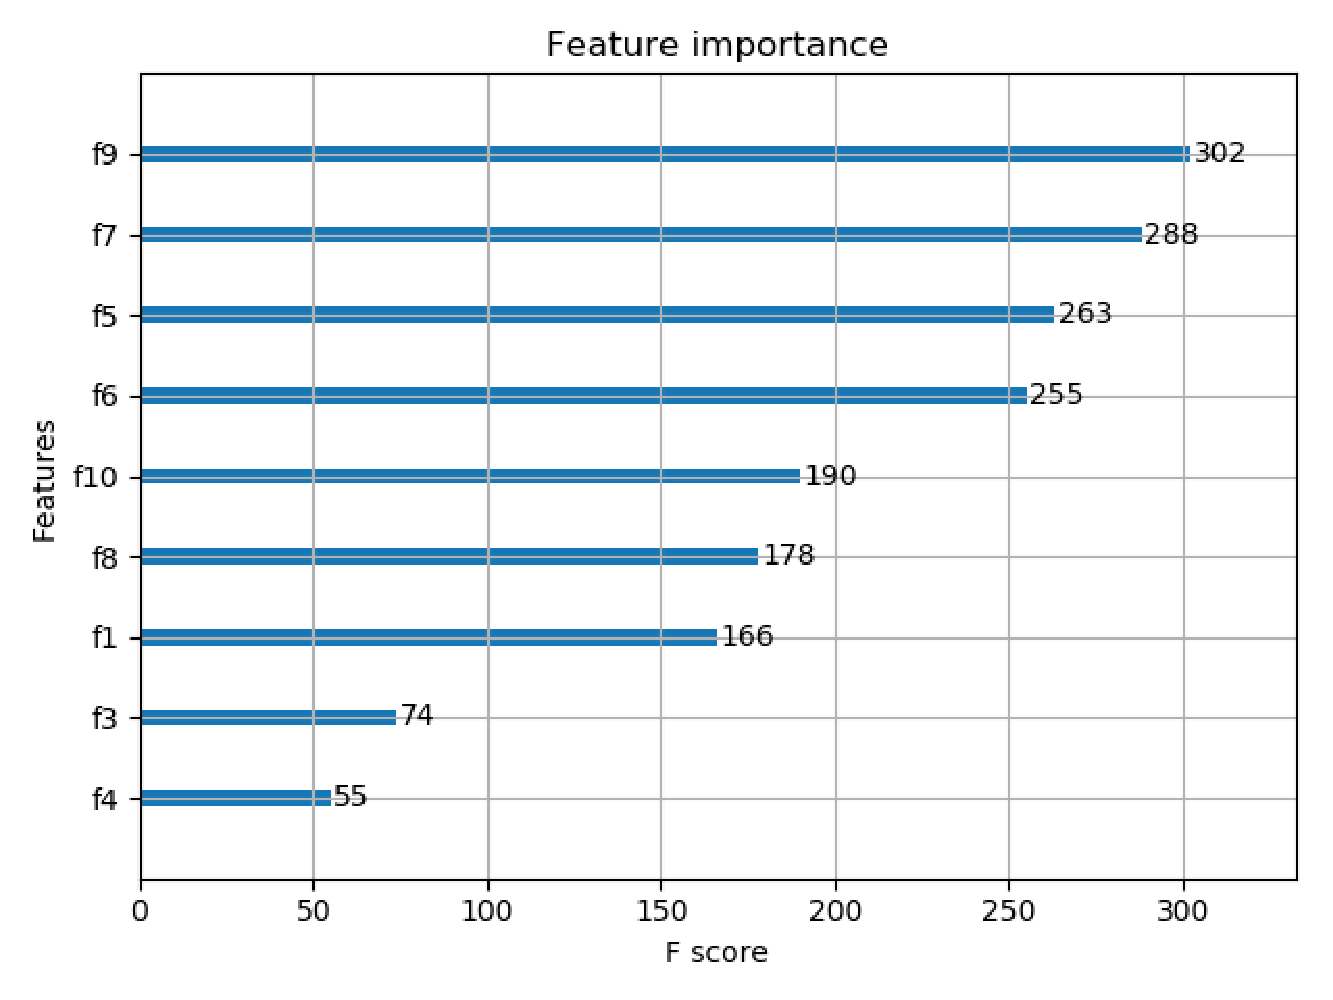
\includegraphics[width=0.5\columnwidth]{./figures/morning_rank.pdf} &  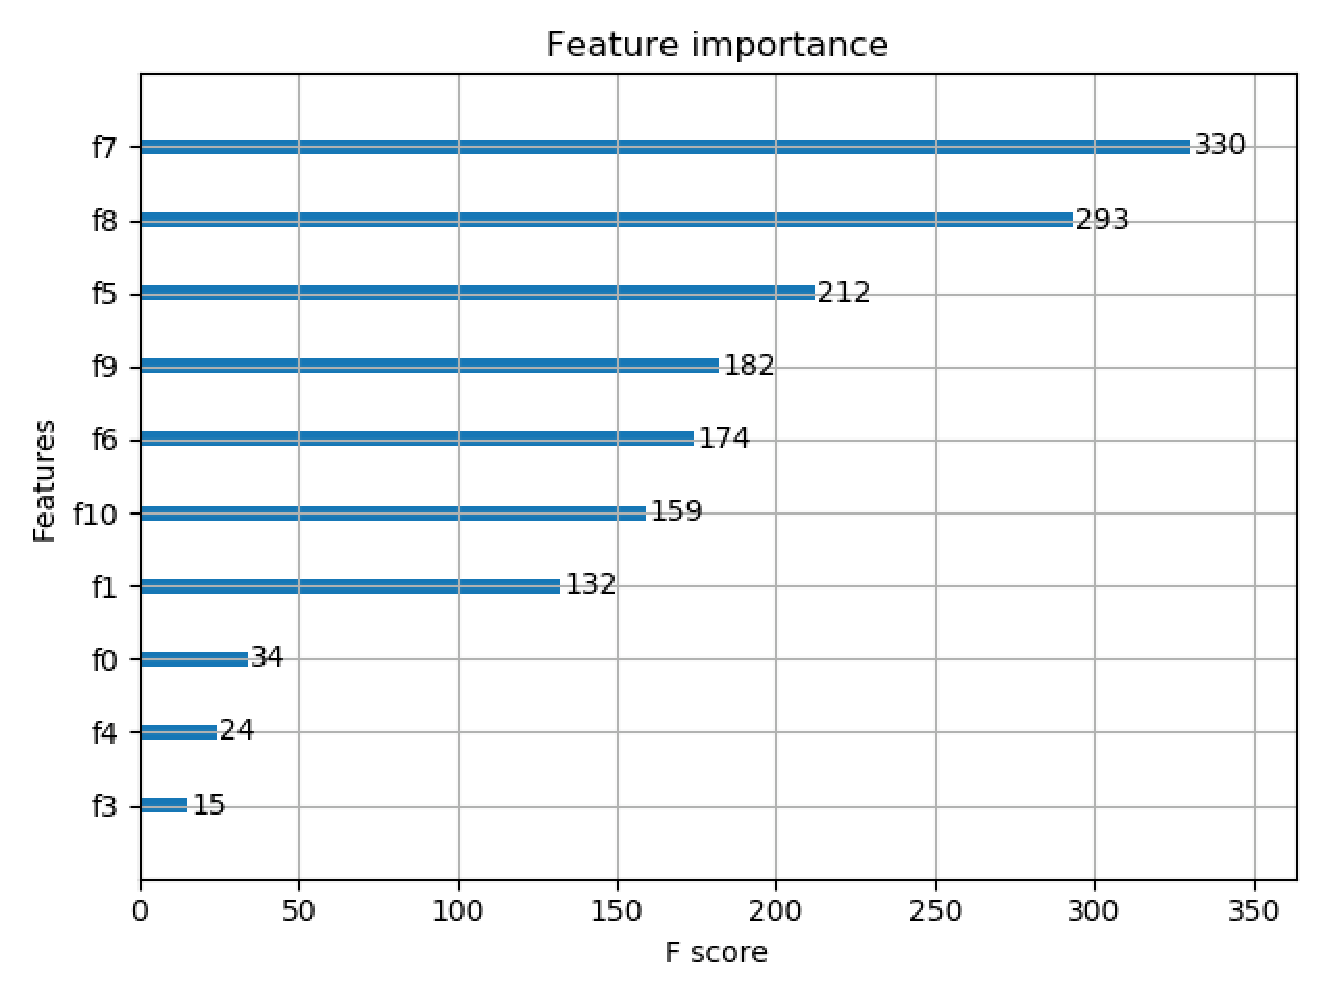
\includegraphics[width=0.5\columnwidth]{./figures/evening_rank.pdf} \\
		(a) Morning\_Rank & (b) Evening\_Rank \\
	\end{tabular}
	\centering
	\caption{Feature Importance Of Morning \& Evening Prediction}
	\label{fig11}
\end{figure}

\begin{figure}[!htbp]
	\begin{tabular}{cc}
		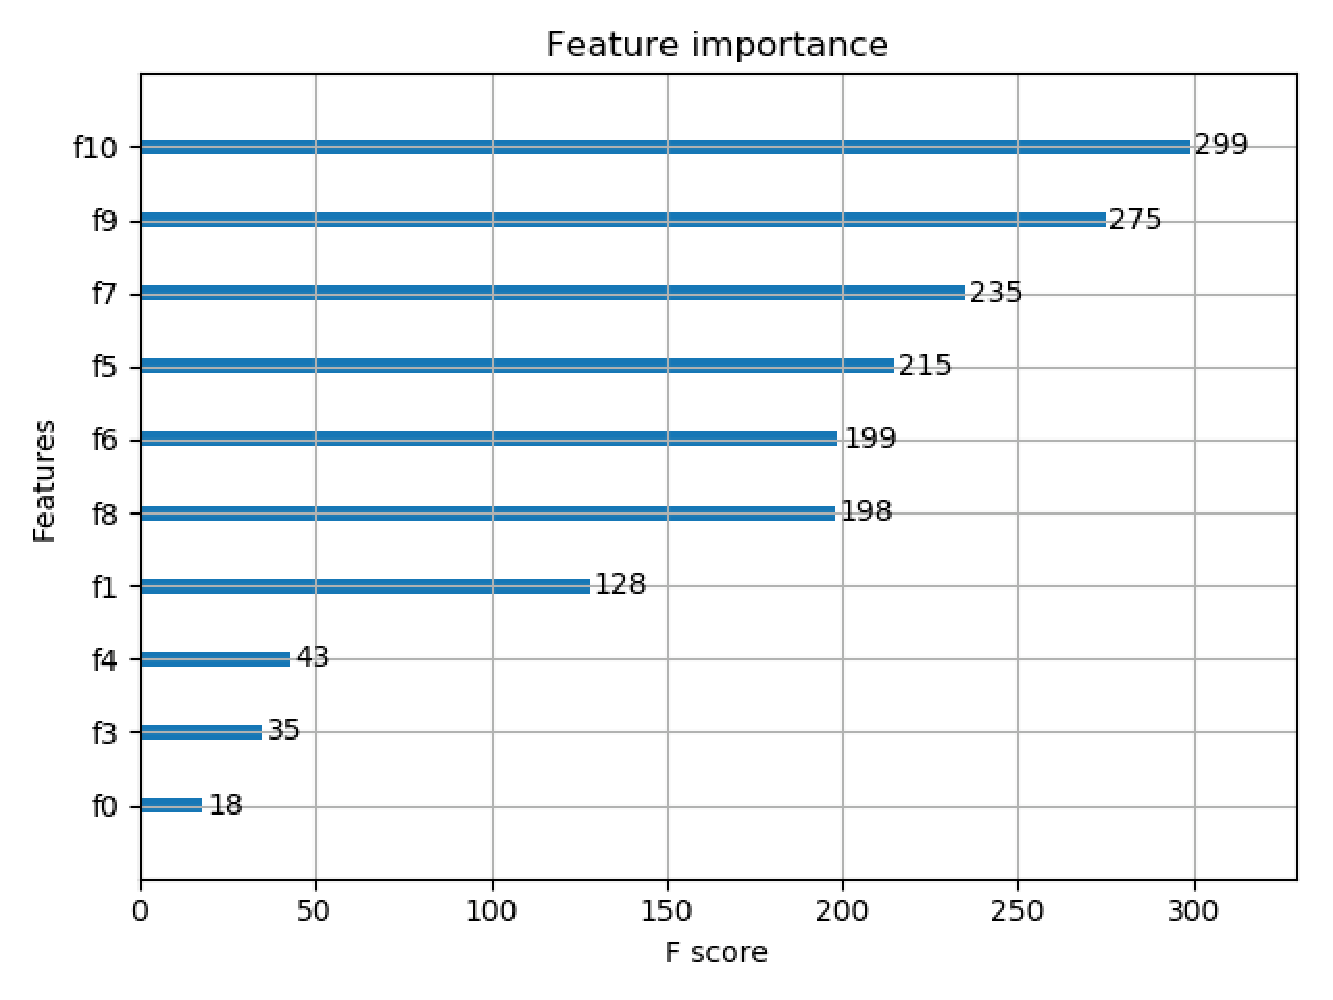
\includegraphics[width=0.5\columnwidth]{./figures/weekday_rank.pdf} &  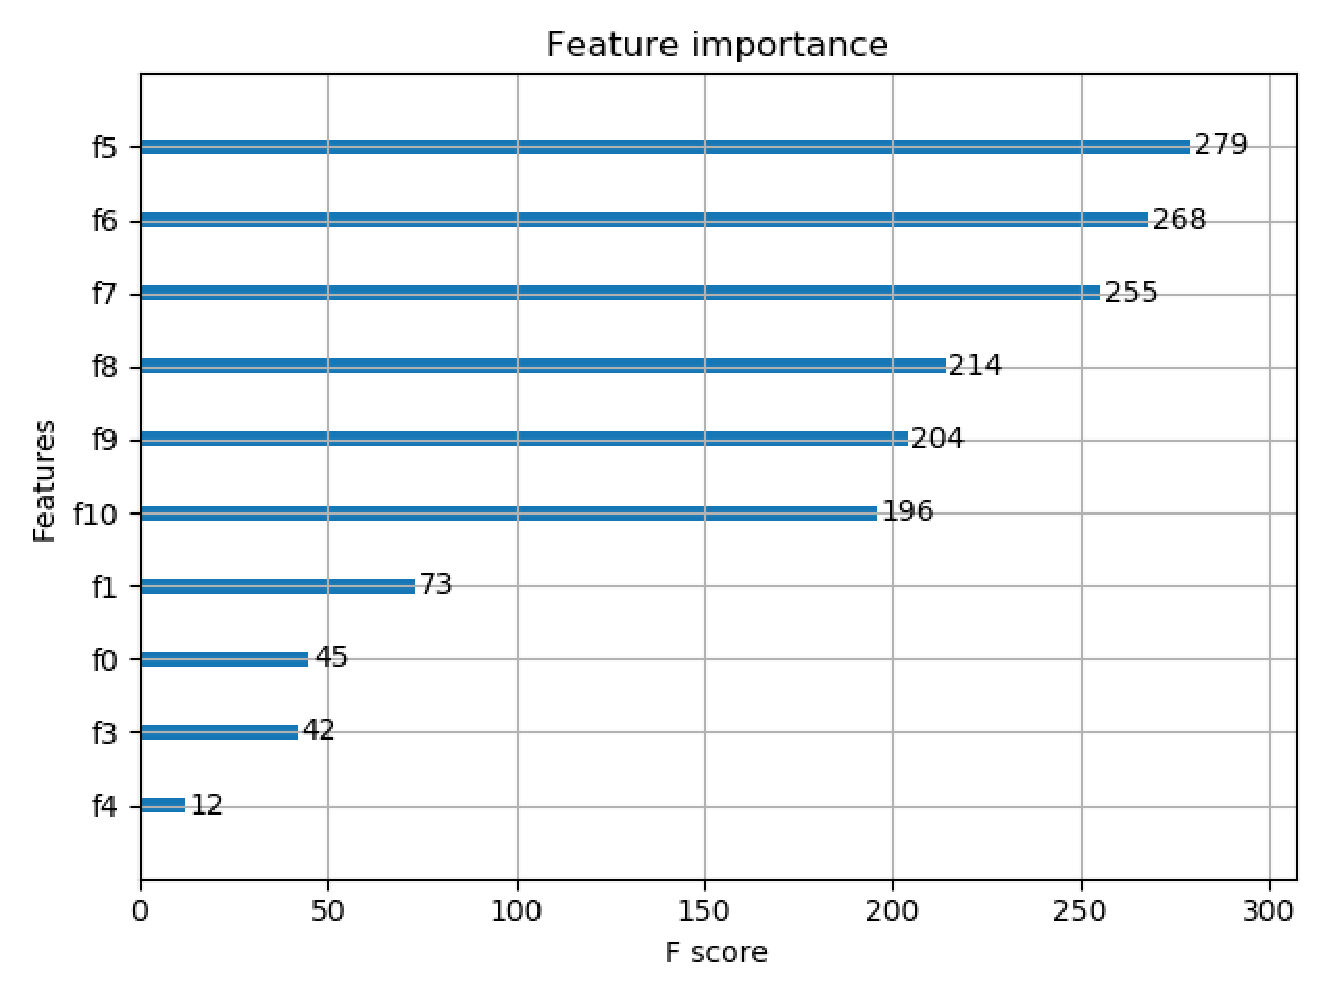
\includegraphics[width=0.5\columnwidth]{./figures/weekend_rank.pdf} \\
		(a) Weekday\_Rank & (b) Weekend\_Rank \\
	\end{tabular}
	\centering
	\caption{Feature Importance Of Weekday \& Weekend Prediction}
	\label{fig12}
\end{figure}

\section{Conclusion}
In this paper, we propose the Feature To Explain LSTM (FTE-LSTM) framework for use rate prediction of charging stations and explain the feature importance correlated to classification result. We study on some important features including station's surrouding POIs, charing price, charging port types and whether it's for private or public use. We assume that use rate values will vary in different area districts and different time frames, so we separate our dataset into urban, suburb area and different time frames to make further analyses. In experiments, we employ our model on two tasks, including districts use\_rate prediction and time frames use\_rate prediction, when compared to traditional classifiers, our model can obtain relatively favourable results. Furthermore, we conduct feature importance ranking for each task, and find that important POIs have greater impact on stations use rate than other kinds of features. At the same time, the most influential POI may vary in different districts or time frames, which indicates that when planning charging stations placement, operators should consider spatio and temporal factors together to make the best decision.

There is still a lot of work to be continued in the future. First, we only consider four main types of features that might affect stations' use rate, many other important features also need to be extracted and included. Second, we don't make fully use of rich spatio temporal informaton behind our dataset, we will dig into it deeper in our future work. Finally, our model still needs optimization and apply a more useful ranking algorithm to get better accuracy and ranking results.
%
% ---- Bibliography ----
%
% BibTeX users should specify bibliography style 'splncs04'.
% References will then be sorted and formatted in the correct style.
%
% \bibliographystyle{splncs04}
% \bibliography{mybibliography}
%
\bibliographystyle{IEEEtran}
\bibliography{reference}
\end{document}
